\section{Task: Parallelizing the Mandelbrot set using MPI [20 Points]}
%Comment the performance observed in the graph perf.pdf in your report. Give a suggestion to improve the performance.
In \ref{fig:mandel} you can see the performance of the Mandelbrot set spread out over different number of processes. This shows how much work each thread has to do depending on the number of processes. If we have more than two processes we can clearly see that the workload is unevenly distributed across the processes. This imbalance is caused by the fact that different regions of the complex plane need varying numbers of iterations to determine if a point is part of the mandelbrot set. For higher number of processes we can see that workload is distributed more evenly, yet there are still processes that do very little compared to others.
\begin{figure}[H]
	\centering
	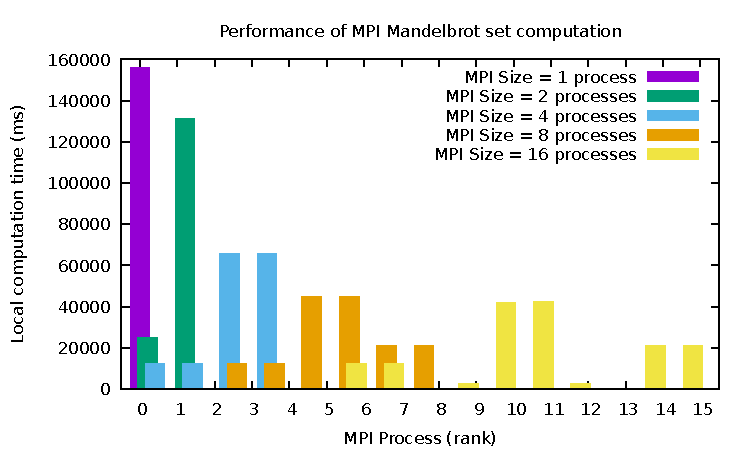
\includegraphics[width=0.8\textwidth]{../media/perf.pdf}
	\caption{MPI Performance of the Mandelbrot on the Rosa Cluster for 1 to 16 Processes}
	\label{fig:mandel}
\end{figure}

In order to improve the performance a different partitioning scheme with different sized grids could be used. I would make the number of grids higher in computational demanding areas and as a result decrease the size of this grids in said area. Furthermore the grids would be bigger for less computational demanding areas. This would result in an improved workload balanced across all the processes.
